\section{Introducción al Machine Learning}
\subsection{Tareas básicas del Machine Learning}
\subsubsection*{¿Qué es el Machine Learning?}
\begin{itemize}[label=\color{red}\textbullet, leftmargin=*]
	\item \color{lightblue}Definición de Machine Learning
\end{itemize}
"Descubrir regularidades en datos mediante el uso de algoritmos, y mediante el uso de esas regularidades realizar alguna acción" (C. M. Bishop)
\begin{itemize}[label=\color{red}\textbullet, leftmargin=*]
	\item \color{lightblue}Tareas básicas
\end{itemize}
Fundamentalmente cuatro:
\begin{itemize}[label=\color{lightblue}\textbullet]
	\item Clasificación
	\begin{itemize}[label=\color{lightblue}$\to$]
		\item \textbf{Detección de spam:} Se trata de clasificar, mediante identificación de patrones, los correos electrónicos como spam o no spam.
		\item \textbf{Detección de fraudes:} Distinción entre transacciones legítimas y sospechosas basándose en patrones y características relevantes.
		\item \textbf{Análisis de sentimientos:} Los algoritmos de clasificación pueden utilizarse para determinar el sentimiento expresado en un texto, como positivo, negativo o neutro. Esto es útil para el análisis de opiniones en redes sociales, comentarios de clientes, revisiones de productos, etc.
		\item \textbf{Detección de objetos en imágenes:} Especialmente útil en la conducción de coches autónomos.
	\end{itemize}
	\item Regresión
	\begin{itemize}[label=\color{lightblue}$\to$]
		\item \textbf{Estimación de la demanda de un producto:} Predicción de la demanda de un producto en función de variables como el precio, la publicidad, las tendencias del mercado, entre otras.
		\item \textbf{Predicción de la contaminación atmosférica:} Utilizando datos históricos de contaminantes, meteorología y otras variables relevantes, se puede aplicar la regresión para predecir los niveles de contaminación en una ubicación específica.
		\item \textbf{Análisis de la relación entre variables económicas:} La regresión puede utilizarse para explorar la relación entre variables económicas, como el crecimiento del PIB y el desempleo, con el fin de entender mejor su interdependencia y tomar decisiones políticas o empresariales informadas.
	\end{itemize}
	\item Agrupamiento
	\item Asociación
\end{itemize}
\begin{itemize}[label=\color{red}\textbullet, leftmargin=*]
	\item \color{lightblue}Tarea de agrupación en Machine Learning
\end{itemize}
El \textbf{agrupamiento} o \textbf{clustering} consiste en detectar agrupaciones en datos \underline{no etiquetados} empleando alguna media  de similitud entre ellas. El objetivo es descubrir patrones y estructuras dentro de los datos.

Algoritmos populares para clustering incluyen el K-Means, el DSCAN, el clustering jerárquico y Mapas Autoorganizados (SOM).

\bu{Ejemplo K-Means}
\begin{center}
	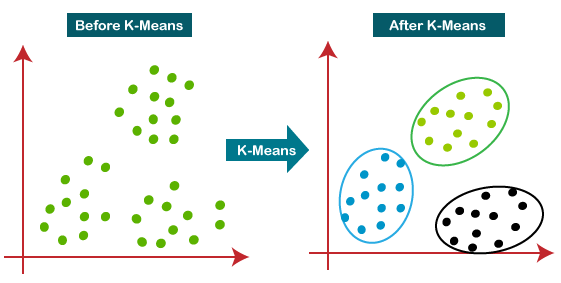
\includegraphics[scale=0.7]{"Temas/Tema 1/K-means.png"}
\end{center}
\begin{itemize}[label=\color{red}\textbullet, leftmargin=*]
	\item \color{lightblue}Tarea de asociación en Machine Learning
\end{itemize}

La tarea de \textbf{asociación} se centra en descubrir reglas de asociación entre eventos en un conjunto de datos, lo que significa identificar qué elementos tienden a aparecer juntos en dichos eventos. El objetivo es revelar después del afeitado, hay un 80\% de posibilidades de que el cliente compre también crema de afeitado.

La asociación es una tarea \underline{no supervisada}, los datos a menudo provienen de transacciones o eventos, y no se requieren etiquetas previas.

Algoritmos como Apriori se utilizan comúnmente para generar reglas de asociación en los datos, reglas como "Si A, entonces B". Estas reglas se utilizan en análisis de mercado y sistemas de recomendación.
\subsection{Generalización: subajuste y sobreajuste}
\subsubsection{Planteamiento del problema}
En el contexto del Machine Learning, el \textbf{conjunto de hipótesis} se refiere a un conjunto de funciones o modelos matemáticos que se utilzian para aproximar una relación desconocida entre las \textbf{entradas $(x)$} y las \textbf{salidas deseadas o targets $(t)$} de un conjunto de datos.

Cada hipótesis representa una posible aproximación de la relación subyacente en los datos.

El objetivo del \textbf{aprendizaje supervisado} es encontrar la hipótesis que mejor se ajuste a los datos de entrenamiento manteniendo la capacidad de hacer predicciones precisas para datos nuevos \textbf{(capacidad de generalización)}.

\begin{center}
	\begin{tikzpicture}
		% Define los nodos
		\node (A) at (0,0) {$x_j$};
		\node[draw=blue, right=2cm of A, text width=2cm, fill=lightblue!10] (B) {\begin{center}
				Máquina de \\ Aprendizaje \\ $y(x,w)$
		\end{center}};
		\node[right=2cm of B] (C) {$y(x_j,w)$};
		
		% Dibuja las flechas
		\draw[double -latex=4pt colored by lightblue and lightblue!10] (A) -- (B);
		\draw[double -latex=4pt colored by lightblue and lightblue!10] (B) -- (C);
	\end{tikzpicture}
\end{center}

\begin{itemize}[label=\color{red}\textbullet, leftmargin=*]
	\item \lb{Necesario: Conjunto de entrenamiento}
	
	Pares: $\{x_j,t_j\}$ con $j=1,2,\dots,N$.\\
	$x_j=\{x_{j1},x_{j2},\dots,x_{jD}\}$ entrada $j$-ésima; vector con $D$ \textbf{componentes o características}.\\
	$t_j=\{x_{j1},x_{j2},\dots,x_{jT}\}$ target $j$-ésimo; vector con $T$ componentes.
	\item \lb{Objetivo: Aprendizaje supervisado}
	
	Encontrar las \textbf{variables o pesos} del modelo $(\mathbf{w})$ que resuelvan el problema: $y(x_j,\mathbf{w})\eqsim t_j$ para $j=1,2,\dots,N$. A esta tarea se la denomina \textbf{entrenamiento}.
\end{itemize}
\bu{Ejemplo: Problema de \textbf{regresión}}

$y=\sin(2\pi x)+n(x)$, donde $n(x)$ es un ruido gausiano pequeño.

\begin{wrapfigure}[3]{l}{0.3\textwidth}
	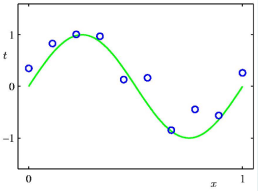
\includegraphics{"Temas/Tema 1/Entrenamiento.png"}
\end{wrapfigure}

Conjunto de entrenamiento: $\{x_j,t_j\}_{j=1}^{N=10}$

\begin{flushright}
	\begin{tikzpicture}
		% Define los nodos
		\node (A) at (0,0) {$x_j$};
		\node[draw=blue, right=2cm of A, text width=2cm, fill=lightblue!10] (B) {\begin{center}
				Máquina de \\ Aprendizaje \\ $y(x,w)$
		\end{center}};
		\node[right=2cm of B] (C) {$y(x_j,w)$};
		
		% Dibuja las flechas
		\draw[double -latex=4pt colored by lightblue and lightblue!10] (A) -- (B);
		\draw[double -latex=4pt colored by lightblue and lightblue!10] (B) -- (C);
	\end{tikzpicture}
\end{flushright}

Aproximador polinómico: $y(x,\mathbf{w})=w_0+w_1x+w_2x^2+\cdots+x_Mx^M=\sum_{j=0}^{M}x_jx^j$

\begin{itemize}
	\item $M$ es un parámetro que determina la complejidad del modelo (orden del polinomio).
	\item Los parámetros no entrenables que determinan el modelo o el entrenamiento se denominan en Machine Learning \textbf{hiperparámetros}.
\end{itemize}
\subsubsection{Planteamiento de la solución}
Se quiere encontrar las variables del modelos (coeficientes del polinomio) para que éste minimice una función de coste o error, por ejemplo, la función de error SSE ("Sum of Square Error") dada por \[ E(\mathbf{w})=\dfrac{1}{2}\sum_{n=1}^{N}\left\{y(x_n,\mathbf{w})-t_n\right\}^2 \]Existe una solución analítica única mediante álgebra lineal.


\begin{center}
	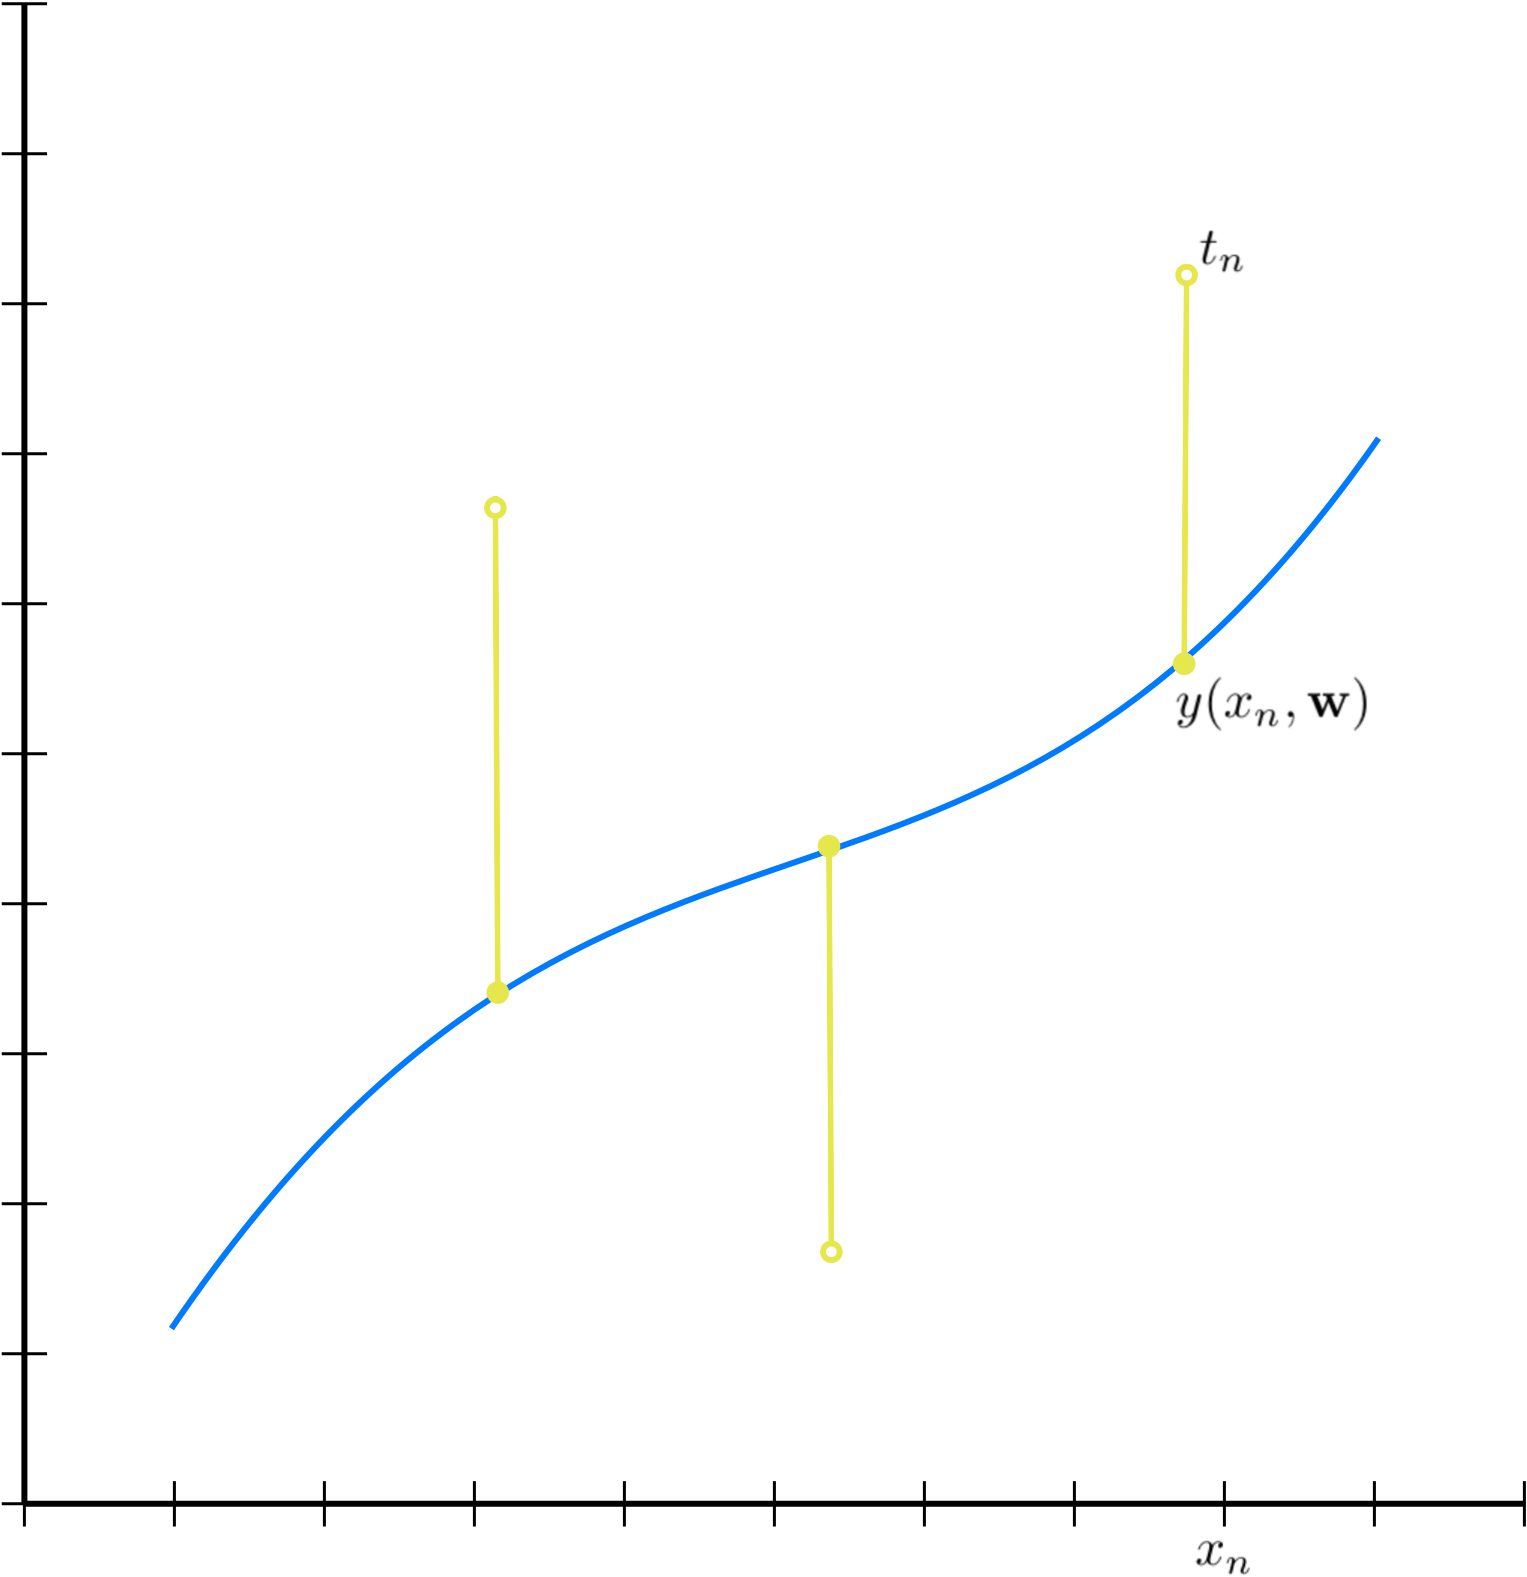
\includegraphics{"Temas/Tema 1/SSE.png"}
\end{center}

\subsubsection{Peligros}
\subsubsection{Subajuste y sobreajuste}

\begin{center}
	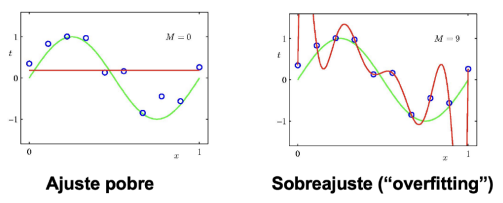
\includegraphics{"Temas/Tema 1/Ajustes.png"}
\end{center}
\subsubsection{Complejidad del modelo vs número de datos}
\begin{minipage}{0.6\textwidth}
	\begin{itemize}[label=\color{red}\textbullet, leftmargin=*]
		\item \color{lightblue}Comoportamiento con $M(N\text{ fijo})$
	\end{itemize}
	Fijado $N$, la complejidad del modelo determina la generalización
\end{minipage}\qquad\begin{minipage}{0.4\textwidth}
	\includegraphics{"Temas/Tema 1/Screenshot001"}
\end{minipage}

\begin{minipage}{0.4\textwidth}
	\begin{itemize}[label=\color{red}\textbullet, leftmargin=*]
		\item \color{lightblue}Comportamiento con $N$ ($M$ fijo)
	\end{itemize}
	Fijado $N(M=9)$, $N$ condiciona la solución del problema: si es bajo, se puede sobreajustar, si es alto (con relación a la dimensión) se reduce el sobreajuste.
\end{minipage}\qquad\begin{minipage}{0.4\textwidth}
	\begin{center}
		\includegraphics{"Temas/Tema 1/Screenshot009"}
	\end{center}
\end{minipage}
\subsubsection{Conclusión}
Hay que limitar la complejidad del modelo acorde con el número de datos disponibles.

En número de muestras ($N$) suele ser un parámetro fijo condicionado por el problema.

Hay que lidiar con el compromiso entre la complejidad y el error de generalización.

\subsubsection{Descomposición sesgo-varianza. Coste cuadrático}
\begin{itemize}[label=\color{red}\textbullet, leftmargin=*]
	\item \color{lightblue}Solución óptima
\end{itemize}
En el contexto de machine learning y desde un punto de vista teórico, los datos de un problema se considera extraídos de una disposición $p(\mathbf{x},t)$. Definamos: 
\begin{itemize}
	\item Salida del modelo regresor: $y(\mathbf{x})$, aporta la solución $(y(\mathbf{x})\eqsim t)$.
	\item Coste cuadrático para una entrada $\mathbf{x}$: $L=(y(\mathbf{x})-t)^2$.
	\item Coste cuadrático promedio (MSE): \begin{align}
		E[L]&=\int_\mathbf{x}\int_t L(t,y(\mathbf{x}))p(\mathbf{x},t)\dt\mathrm{d}\mathbf{x}\\
		&=\int_\mathbf{x}\int_t(y(\mathbf{x})-t)^2p(\mathbf{x},t)\dt\mathrm{d}\mathbf{x}
	\end{align}
\end{itemize}

El término cuadrático de la Ecuación (1), se puede escribir como \[\begin{aligned}
	\{y(\mathbf{x})-t\}^2&=\{y(\mathbf{x})-E_t[t|\mathbf{x}]+E_t[t|\mathbf{x}]-t\}^2\\
	&=\{y(\mathbf{x})-E_t[t|\mathbf{x}]\}^2+\{E_t[t|\mathbf{x}]-t\}^2+2\{y(\mathbf{x})-E_t[t|\mathbf{x}]\}\{E_t[t|\mathbf{x}]-t\}
\end{aligned}\] que insertado en (1) produce \[
E[L]=\int\mathbf{x}\int_t\{y(\mathbf{x})-E_t[t|\mathbf{x}]\}^2p(\mathbf{x},t)\dt\mathrm{d}\mathbf{x}+\int_\mathbf{x}\int_t\{E_t[t|\mathbf{x}]-t\}^2P(\mathbf{x},t)\dt\mathrm{d}\mathbf{x}+\int_\mathbf{x}\int_t2\{y(x)-E_t[t|\mathbf{x}]\}\{E_t[t|\mathbf{x}]-t\}p(\mathbf{x},t)\dt\mathrm{d}\mathbf{x}
\] y realizando la integral sobre $t$, se obtiene  \begin{align}
	E[L]=\int_{\mathbf{x}}\{y(\mathbf{x})-E_t[t|\mathbf{x}]\}^2p(\mathbf{x})\mathrm{d}\mathbf{x}+\int_\mathbf{x}\mathrm{var}(t|\mathrm{x})+0 
\end{align}
\begin{itemize}
	\item El primer término queda así debido a que el integrando no depende de $t$.
	\item El segundo término representa la variabilidad intrínseca del target $t$ promediada sobre $t$ y $\mathbf{x}$, y el valor mínimo posible del coste esperado ($E[L]$). Se considera, por tanto, un ruido irreducible del problema.
	\item El tercer término se anula ya que al realizar la integral sobre $t$ se tiene \begin{align*}
		\int_t2\{y(\mathbf{x})-E_t[t|\mathbf{x}]\}\{E_t[t|\mathbf{x}]-t\}p(\mathbf{x},t)\dt&=2\{y(\mathbf{x})-E_t[t|\mathbf{x}]\}\int_t\{E_t[t|\mathbf{x}]-t\}p(\mathbf{x},t)\dt\\
		&=E_t[t|\mathbf{x}]-E_t[t|\mathbf{x}]\\
		&=0
	\end{align*}
\end{itemize}
Como el segundo término de (3) no depende de nuestro regresor $y(\mathbf{x})$, la solución óptima que minimiza $E[L]$, y que llamaremos $h(\mathbf{x})$, es: \[ \boxed{h(\mathbf{x})=E_t[t|\mathbf{x}]} \]que anula el primer término de (3).
\begin{itemize}[label=$-$]
	\item Representación gráfica de la solución óptima (mínimo MSE). Ejemplo unidimensional.
	\item Como acabamos de ver, la solución es $y(x)=E_t[t|x]$, es decir, $h(x)$.
\end{itemize}
\begin{center}
	\includegraphics[scale=0.7]{"Temas/Tema 1/Screenshot010"}
\end{center}
En la práctica, \textbf{nunca tendremos infinitas muestras}, sino un conjuto finito $D$ de $N$ datos: $D=\{x_j,t_h\}_{j=1}^{N}$. Por esto, no podemos conocer $h(\mathbf{x})$ con exactitud.

\begin{minipage}{0.5\textwidth}
	Si modelamos $h(\mathbf{x})$ con una función paramétrica $y(\mathbf{x}, \mathbf{w})$ gobernada por el vector $\mathbf{w}$, entonces la incertidumbre del modelo se puede tratar de dos formas:
	\begin{enumerate}[label=\arabic*)]
		\item Considerando un único conjunto de datos $D$, de forma que la incertidumbre se expresa tratando $\mathbf{w}$ como una variable aleatoria (con una distribución a posteriori de $\mathbf{w}$, teoría bayesiana).
		\item Considerando que se dispone de un gran número de conjuntos de datos diferentes, cada uno con $N$ muestras extraídas independientemente de $p(\mathbf{x}, t)$, de forma que para cada uno de ellos, se obtiene –mediante algún algoritmo de entrenamiento– un predictor $y(\mathbf{x}, D)$ definido por un único vector $\mathbf{w}$ (estimación única para cada $D$).
	\end{enumerate}
\end{minipage}\qquad\begin{minipage}{0.45\textwidth}
	\begin{center}
		\includegraphics{"Temas/Tema 1/Screenshot011"}
	\end{center}
\end{minipage}
Siguiendo la segunda opción, para cada conjunto $D$ y muestra $\mathbf{x}$, se obtiene un error dado por: \[ \{y(\mathbf{x},\mathbf{D})-\mathbf{h(x)}\}^2 \]
Introduciendo el promedio sobre $D$ de nuestro regresor para $\mathbf{x}$, podemos re-escribir el error como \[ \{y(\mathbf{x},D)-E_D[y(\mathbf{x},D)]-h(\mathbf{x})\}^2=\{y(\mathbf{x},D)-E_D[y(\mathbf{x},D)]\}^2+\{E_D[y(\mathbf{x},D)]-h(\mathbf{x})\}^2+2\{y(\mathbf{x},D)-E_D[y(\mathbf{x},D)]\}\{E_D[y(\mathbf{x},D)]-h(\mathbf{x})\} \]
Promediando con respecto a $D$, se anula el tercer término y se obtiene el \textbf{error esperado para la muestra $x$}: \begin{align}
	\boxed{E_D[\{y(\mathbf{x},D)-h(\mathbf{x})\}^2]=\underbrace{E_D[\{y(\mathbf{x},D)-E_D[y(\mathbf{x},D)]\}^2]}_{\mathrm{varianza}}+\underbrace{\{E_D[y(\mathbf{x},D)]-h(\mathbf{x})\}^2}_{(\mathrm{sesgo})^2}}
\end{align}
\begin{itemize}[label=\color{red}\textbullet, leftmargin=*]
	\item \color{lightblue}Error esperado total: sesgo, varianza y ruido
\end{itemize}
Hasta ahora tenemos considerado el error producido por una única muestra $\mathbf{x}$. Incluyendo (4) en el primer término de (3), se obtiene el \textbf{error global esperado} \begin{center}
	\fbox{Error esperado = varianza + $(\mathrm{sesgo})^2$ + ruido}
\end{center}
donde \[ \mathrm{varianza}=\int_\mathbf{x}E_D[\{y(\mathbf{x},D)-E_D[y(\mathbf{x},D)]\}^2]p(\mathbf{x})\dbx \] es la diferencia cuadrática entre las predicciones de nuestro modelo y la media de dichas predicciones; \[ (\mathrm{sesgo})^2=\int_\mathbf{x}\{E_D[y(\mathbf{x},D)]-h(\mathbf{x})\}^2p(\mathbf{x})\dbx \]es la diferencia entre la predicción esperada de nuestro modelo y los valores verdaderos; y \[ \mathrm{ruido}=\int_\mathbf{x}\int_t\{h(\mathbf{x})-y\}^2p(\mathbf{x},t)\dt\dbx \]es el error irreductible que siempre está presente. Es el segundo término de (3).
\subsubsection*{Representaciones gráficas}
\begin{itemize}[label=\color{red}\textbullet, leftmargin=*]
	\item \color{lightblue}Error esperado vs Complejidad
\end{itemize}
\begin{center}
	\includegraphics{"Temas/Tema 1/Screenshot012"}
\end{center}
\begin{itemize}
	\item Modelos complejos (alta capacidad, flexibles) producen varianzas elevadas y sesgos bajos
	\item Modelos simples (baja capacidad, rígidos) producen varianzas bajas y sesgos elevados
\end{itemize}
\begin{itemize}[label=\color{red}\textbullet, leftmargin=*]
	\item \color{lightblue}Sesgo
\end{itemize}
Sea $f(\mathbf{x})$ una función desconocida que queremos aproximar, la llamaremos \textit{"true function"}. Supongamos que tenemos diferentes conjuntos de entrenamiento extraídos de función de distribución definida como "$f(\mathbf{x})$ + noise". La siguiente figura muestra tres regresores lineales, uno para cada conjunto de entrenamiento.
\begin{center}
	\includegraphics{"Temas/Tema 1/Screenshot013"}
\end{center}

\begin{itemize}[label=\color{red}\textbullet, leftmargin=*]
	\item \color{lightblue}Varianza
\end{itemize}
En este caso, las regresiones se realizan perfectamente mediante árboles de decisión sin podar. Cada uno, se ajusta perfectamente a los datos.
\begin{center}
	\includegraphics{"Temas/Tema 1/Screenshot014"}
\end{center}
\begin{itemize}[label=\color{red}\textbullet, leftmargin=*]
	\item \color{lightblue}Compromiso sesgo-varianza
\end{itemize}
\begin{center}
	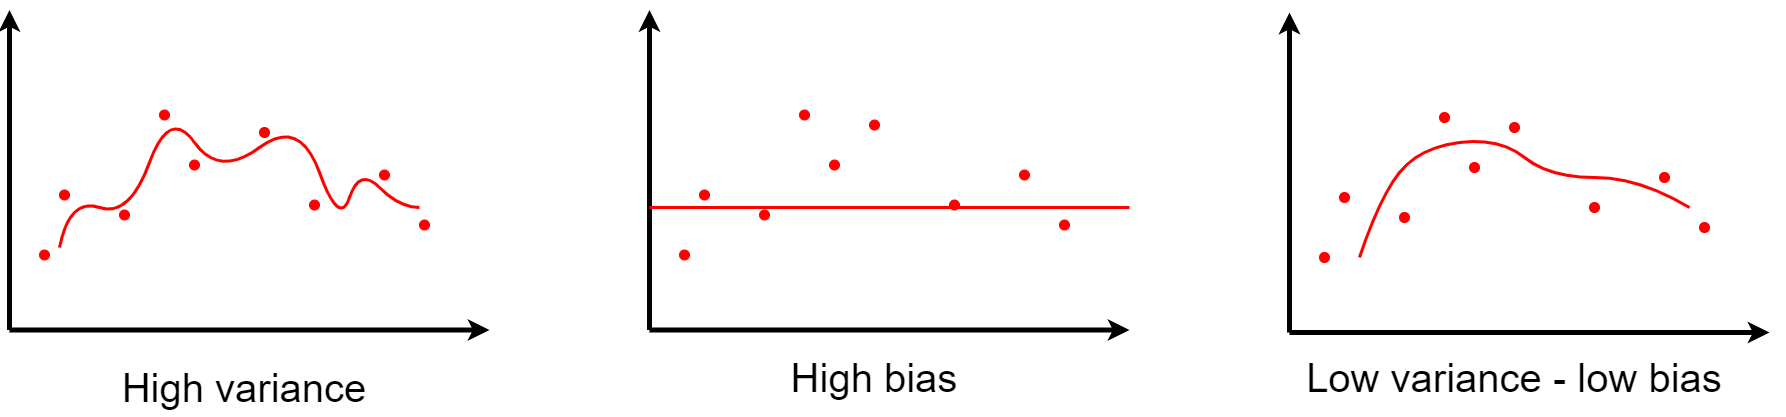
\includegraphics[width=\linewidth]{"Temas/Tema 1/sesgo-varianza.drawio.png"}
\end{center}

\begin{minipage}{0.5\textwidth}
	\begin{itemize}
		\item Mismo ejemplo de regresión considerado anteriormente.
		\item 100 conjuntos de datos, cada uno con 25 muestras. Se realizan 100 entrenamientos.
		\item Regresores: mezclas de 24 guasianas.
		\item $\lambda$ parámetro que determina la complejidad del modelo. Aumenta hacia abajo.
		\item En la primer columna, se muestran 20 entrenamientos (modelos).
		\item Resultados:
		\begin{itemize}
			\item Primera fila: complejidad baja, varianza pequeña y sesgo grande.
			\item Última fila: complejidad alta, varianza grande y sesgo bajo.
			\item Fila centro: solución intermedia. Mejor compromiso sesgo-varianza.
		\end{itemize}
	\end{itemize}
\end{minipage}\qquad\begin{minipage}{0.45\textwidth}
	\begin{center}
		\includegraphics[width=\linewidth]{"Temas/Tema 1/Screenshot015"}
	\end{center}
\end{minipage}
\subsubsection{Algunas técnicas de generalización}
\subsubsection*{¿Cómo evitar el \textbf{sobre}-ajuste?}
\begin{itemize}
	\item \textbf{"Early stopping":} Se detiene el entrenamiento del modelo antes de que alcance la convergencia total en los datos de entrenamiento. Se emplea un conjunto de parada.
	\item \textbf{Regularización L1 y L2} (Regresión Ridge y Lasso): Se agregan términos de penalización (normas L1 ó L2 de los coeficientes del modelo) a la función de pérdida durante el entrenamiento. Son técnicas \textbf{'Weight decay'}.
	\item \textbf{Dropout:} Es una técnica específica para redes neuronales. Durante el entrenamiento aleatoriamente se desactivan (ponen a cero) ciertas neuronas en cada paso. Esto evita que el modelo dependa demasiado de neuronas específicas y promueve una mejor generalización.
	\item \textbf{Aumento de datos:} Se aumenta el tamaño del conjunto de datos mediante técnicas como la rotación, la inversión y el recorte de imágenes. Esto ayuda a exponer al modelo a una mayor variedad de datos y reduce el riesgo de sobreajuste.
	\item \textbf{Feature Selection:} La selección adecuada de características es esencial para evitar el sobreajuste. Eliminar características irrelevantes o altamente correlacionadas puede reducir la complejidad del modelo y mejorar su generalización.
	\item \textbf{Ensemble learning:} Combina múltiples modelos más simples y menos propensos al sobreajuste. El Bagging (Bootstrap Aggregating) y el Boosting son ejemplos de ensemble learning.
\end{itemize}
\subsubsection*{¿Cómo evitar el \textbf{sub}-ajuste?}
\textbf{Evitar el sub-ajuste es tan importante como evitar el sobre-ajuste.}
\begin{itemize}
	\item Aumentar la complejidad del modelo.
	\item Aumentando el tiempo de entrenamiento.
	\item Añadiendo más características.
	\item Reducir la regularización.
\end{itemize}
\subsubsection{Evitar el sobreajuste: "early stopping"}
\begin{itemize}[label=\color{lightblue}$\RHD$]
	\item \textbf{Sobreentrenamiento:} demasiados ciclos adaptan en exceso la red a las muestras de entrenamiento, no generalizando bien.
\end{itemize}
Para evitarlo (mantener la generalización), se emplea un conjunto adicional, extraído del conjunto de entrenamiento llamado \textbf{conjunto de validación} (en este caso, actúa como conjunto de parada)
\begin{center}
	\includegraphics{"Temas/Tema 1/Screenshot016"}
\end{center}
\subsubsection{Evitar el sobreajuste: "Weight Decay"}
Retomamos el problema de \textbf{regresión}: $y=\sin(2\pi\mathbf{x})+n(\mathbf{x})$, donde $n(\mathbf{x})$ es un ruido gausiano pequeño.

\begin{wrapfigure}[3]{l}{0.3\textwidth}
	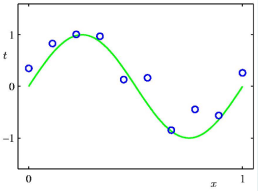
\includegraphics{"Temas/Tema 1/Entrenamiento.png"}
\end{wrapfigure}

Conjunto de entrenamiento: $\{x_j,t_j\}_{j=1}^{N=10}$

\begin{flushright}
	\begin{tikzpicture}
		% Define los nodos
		\node (A) at (0,0) {$x_j$};
		\node[draw=blue, right=2cm of A, text width=2cm, fill=lightblue!10] (B) {\begin{center}
				Máquina de \\ Aprendizaje \\ $y(x,w)$
		\end{center}};
		\node[right=2cm of B] (C) {$y(x_j,w)$};
		
		% Dibuja las flechas
		\draw[double -latex=4pt colored by lightblue and lightblue!10] (A) -- (B);
		\draw[double -latex=4pt colored by lightblue and lightblue!10] (B) -- (C);
	\end{tikzpicture}
\end{flushright}

Aproximador polinómico: $y(x,\mathbf{w})=w_0+w_1x+w_2x^2+\cdots+x_Mx^M=\sum_{j=0}^{M}x_jx^j$

\hspace{1cm}

\begin{itemize}[label=\color{red}\textbullet, leftmargin=*]
	\item \color{lightblue}Técnica de regularización
\end{itemize}
Valores de los \underline{pesos} para varios $M$
\begin{center}
	\includegraphics[width=\linewidth]{"Temas/Tema 1/Screenshot017"}
\end{center}
\textbf{"Weight Decay":} Se regulariza la solución mediante la minimización adicional (cuadrática) de los pesos \[ \tilde{E}(\mathbf{w})=\dfrac{1}{2}\sum_{i=1}^{N}\{y(x_n,\mathbf{w})-t_n\}^2+\underbrace{\dfrac{\lambda}{2}\|\mathbf{w}\|^2}_{\text{Regularización}} \]
\begin{center}
	\includegraphics[width=\linewidth]{"Temas/Tema 1/Screenshot018"}
\end{center}
\begin{minipage}{0.5\textwidth}
	En la figura, se observa como $\lambda$ determina la generalización de la solución
\end{minipage}\qquad\begin{minipage}{0.45\textwidth}
	\begin{center}
		\includegraphics[width=\linewidth]{"Temas/Tema 1/Screenshot019"}
	\end{center}
\end{minipage}

Una forma sencilla de encontrar el valor óptimo de $\lambda$ (la complejidad del modelo) es mediante la evaluación de las prestaciones del \textbf{Conjunto de Validación} (el mismo conjunto empleado para early-stopping).
\subsection{Evaluación de prestaciones}
Para evaluar las prestaciones (\textbf{rendimiento}) de un modelo de machine learning ya entrenado, se utilizan diversas métricas de evaluación dependiendo del tipo de problema (clasificación, regresión, etc.) y las características del conjunto de datos.

Métricas más comunes:
\begin{itemize}
	\item Problemas de regresión.
	\begin{itemize}
		\item Error cuadrático medio (Mean Square Error, MSE)
		\item Error absoluto medio (Mean Absolute Error, MAE)
		\item Coeficiente de Determinación $R^2$.
	\end{itemize}
	\item Problemas de clasificación.
	\begin{itemize}
		\item Matriz de confusión.
		\item Exactitud (Accuracy)
		\item Precisión (Precision)
		\item Sensibilidad (Recall) y Especificidad (Specificty)
		\item F1-score
		\item ROC
	\end{itemize}
\end{itemize}
\subsubsection{Regresión}
\begin{itemize}
	\item \textbf{Error Cuadrático Medio (MSE):} \[ MSE(\mathbf{w})=\dfrac{1}{N}\sum_{i=1}^{N}\{y(x_n,\mathbf{w})-t_n\}^2 \]
	\item \textbf{Error Absoluto Medio (MAE):} \[ MAE(\mathbf{x})=\dfrac{1}{N}\sum_{i=1}^{N}|y(x_n,\mathbf{w})-t_n| \]
\end{itemize}
En estas fórmulas, $N$ el número total de instancias, $y(x_n,w)$ la salida obtenida del modelo $w$ y $t_n$ la salida real de la instancia $n$. Interpretación de MSE y MAE: A menor error mejor siempre será el modelo.
\begin{itemize}
	\item \textbf{Coeficiente de Determinación $R^2$}
	
	Métrica a utilizar en tareas de regresión. Indica la cantidad proporcional de variación en la variable de respuesta $y$, explicada según las variables independientes $X$. Es una medida adimensional. Toma valores en el intervalo $[0,1]$. Cuanto mayor es el valor, mejor es el ajuste del modelo.
\end{itemize}
La fórmula es: \[ R^2=1-\dfrac{\sum(t_i-y_i)^2}{\sum(y_i-\mu_t)^2}. \] Siendo $t_i$ la salida esperada de la instancia $i,\,y_i$ la salida del modelo para la instancia $i$ y $\mu_t$ la media de los valores de salida de todas las instancias. Interpretación de $R^2$.
\begin{itemize}
	\item Valor entre 0 y 1.
	\item Más cercano a 0 $\longrightarrow$ modelo con poco ajuste.
	\item Más cercano a 1 $\longrightarrow$ modelo con mayor ajuste.
	\item Umbral entre el nivel de ajuste se encuentra superior a 0.5, para algunas áreas superior a 0.75.
\end{itemize}
\subsubsection{Clasificación}
\begin{minipage}{0.5\textwidth}
	Supongamos un problema de clasificación binario con datos bidimensionales positivos (clase P) y negativos (clase N). En la figura anexa, se muestra el espacio de los datos y la frontera real (ideal) del problema.
	
	\hspace{2cm}
	
	Cuando se entrena un modelo con los datos disponibles, se obtendrá una frontera diferente a la ideal, como se muestra en la figura.
\end{minipage}\qquad
\begin{minipage}{0.45\textwidth}
	\begin{center}
		\includegraphics[width=0.3\textheight]{"Temas/Tema 1/Screenshot020"}
	\end{center}
\end{minipage}


El objetivo es conseguir un clasificador que produzca una frontera lo más parecida a la real, es decir, \[ \begin{array}{c}
	VP = P\longrightarrow FN=0\\
	\mathrm{y}\\
	VN=N\longrightarrow FP=0
\end{array} \]

\subsubsection*{¿Cómo medir este parecido?}
Con \textbf{métricas} como:
\begin{itemize}
	\item Matriz de Confusión
	\item Exactitud (Accuracy)
	\item Precisión (Precision)
	\item Sensibilidad (Recall) y Especificidad (Specificty)
	\item F1-score
	\item ROC
\end{itemize}

\begin{itemize}[label=\color{red}\textbullet, leftmargin=*]
	\item \color{lightblue}Matriz de confusión
\end{itemize}
\begin{center}
	\includegraphics{"Temas/Tema 1/Screenshot021"}
\end{center}

\begin{minipage}{0.55\textwidth}
	\begin{itemize}[label=\color{red}\textbullet, leftmargin=*]
	\item \color{lightblue}Exactitud (Accuracy)
\end{itemize}
Es el porcentaje de acierto (con independencia de la clase) \[ \mathrm{Exactitud}=\dfrac{\mathrm{VP}+\mathrm{VN}}{\mathrm{P}+\mathrm{N}} \]
\textbf{Desventaja:} mala métrica para problemas desbalanceados
\begin{itemize}[label=\color{red}\textbullet, leftmargin=*]
	\item \color{lightblue}Precisión (Precision)
\end{itemize}
Es el porcentaje de acierto de las predicciones positivas. \[ \text{Precisión}=\dfrac{\mathrm{VP}}{\mathrm{VP}+\mathrm{FP}}=\dfrac{\mathrm{VP}}{P'} \]
\begin{itemize}[label=\color{red}\textbullet, leftmargin=*]
	\item \color{lightblue}Sensibilidad (Recall)
\end{itemize}
Es el porcentaje de casos positivos detectados \[ \mathrm{Sensibilidad}=\dfrac{\mathrm{VP}}{\mathrm{VP}+\mathrm{FN}}=\dfrac{\mathrm{VP}}{\mathrm{P}} \]
Ejemplo en diagnóstico médico: probabilidad de detectar a un enfermo.\\
También se denomina TPR (True Positive Ratio) o Probabilidad de detección ($P_D$).
\begin{itemize}[label=\color{red}\textbullet, leftmargin=*]
	\item \color{lightblue}Especificidad (Specificity)
\end{itemize}
Es el porcentaje de casos negativos detectados. \[ \mathrm{Especificidad}=\dfrac{\mathrm{VN}}{\mathrm{VN}+\mathrm{FP}}=\dfrac{\mathrm{VN}}{\mathrm{N}} \]
Ejemplo en diagnóstico médico: probabilidad de detectar a un sano.\\
También se denomina TNR (True Negative Ratio).
\end{minipage}\qquad\begin{minipage}{0.4\textwidth}
	\begin{center}
		\includegraphics[width=\linewidth]{"Temas/Tema 1/Screenshot022"}
	\end{center}
\end{minipage}

\subsubsubsection{Interpretación de la Precisión y la Sensibilidad}
\textbf{Conjuntamente } indican si existe un sesgo hacia valores positivos o negativos

\begin{minipage}{0.5\textwidth}
	\textbf{Precisión baja + Sensibilidad alta =} Sesgo hacia la clase de negativos (frontera desplazada hacia la clase de negativos). Se puede tener un 100\% de sensibilidad con una muestra negativa acertada.
	
	\textbf{Precisión alta + Sensibilidad baja =} Sesgo hacia la clase de positivos (frontera desplaza hacia la clase de positivos). Se puede tener un 100\% de precisión con una sola muestra positiva acertada.
	
	Típico de \lb{conjuntos \textbf{desbalanceados}}.
\end{minipage}\qquad\begin{minipage}{0.4\textwidth}
\begin{center}
	\includegraphics[width=\linewidth]{"Temas/Tema 1/Screenshot023"}
\end{center}
\end{minipage}
\begin{itemize}
	\item \textbf{Puntuación F1} (F1 score): La puntuación F1 es la \lb{media armónica} de la precisión y sensibilidad, donde la puntuación de la F1 alcanza su mejor valor en 1 (precisión y sensibilidad perfectas) y el peor en 0.
	\item Esta es una métrica muy utilizada en problemas desbalanceados.
\end{itemize}
Se define como: \[ \mathrm{F1}=2\times\dfrac{\mathrm{sensibilidad}\times\text{precisión}}{\mathrm{sensibilidad}+\text{precisión}} \]
\begin{itemize}[label=\color{red}\textbullet, leftmargin=*]
	\item \color{lightblue}ROC (Receiver Operating Characteristic)
\end{itemize}
Es la representación gráfica de la \textbf{Sensibilidad} vs \textbf{Probabilidad de Falsa Alarma} para un sistema clasificador binario según se varía el umbral de discriminación (valor a partir del cual decidimos que un caso es un positivo).
\begin{itemize}[label=\color{red}\textbullet, leftmargin=*]
	\item \color{lightblue}Probabilidad de Falsa Alarma, FPR
\end{itemize}

Es la probabilidad de detección incorrecta de un negativo, es decir, 1 $-$ (la probabilidad de detección correcta de un negativo). Así \[ \text{Falsa alarma}=1-\text{Especificidad}=1-\dfrac{\mathrm{VN}}{\mathrm{N}}=\dfrac{\mathrm{FP}}{N} \]
\textbf{RECORDAR:}\\
Sensibilidad = TPR ó $P_D$\\
Falsa Alarma = FPR (False Positive Ratio) ó $P_{FA}$
\begin{itemize}[label=\color{red}\textbullet, leftmargin=*]
	\item \color{lightblue}AUC (Área Bajo la Curva)
\end{itemize}
\begin{center}
	\includegraphics[width=\linewidth]{"Temas/Tema 1/ScreenShot024.drawio"}
\end{center}
\begin{center}
	\includegraphics{"Temas/Tema 1/Screenshot025"}
\end{center}
\subsubsubsection{Puntuación Kappa}
La métrica de puntuación kappa $k$ tiene sus orígenes se remontan al campo de la psicología: se utiliza para medir la concordancia entre dos evaluadores o clasificadores humanos a la hora de calificar sujetos. En el área del machine learning se utiliza para medir el rendimiento de la clasificación. Se trata de un coeficiente para medir la concordancia existente en la observación de un fenómeno por dos observaciones distintos \[ k=\dfrac{P_o-P_e}{1-P_e} \]donde:
\begin{itemize}
	\item $P_o$ representa la probabilidad observada de que coincida el modelo con la clase real y se calcula simplemente como las instancias correctamente clasificadas frente al total: $P_o=\dfrac{VP+VN}{N}$
	\item $P_e$ representa la probabilidad de que ambos coincidan por mera casualidad (probabilidad esperada):\\ $P_e=\left(\dfrac{VP+FN}{N}\cdot\dfrac{VP+FP}{N}\right)+\left(\dfrac{FP+VN}{N}\cdot\dfrac{FN+VN}{N}\right)$
\end{itemize}
Interpretación de $k$:
\begin{itemize}
	\item Si el modelo coincide con la realidad será perfecto $k=1$
	\item A partir de 0.6 y/o 0.8 según autor se considera un buen modelo de predicción.
\end{itemize}
\subsubsection{Hold-out}
Las métricas deben evaluarse tras el entrenamiento con \textbf{datos nuevos} para medir la capacidad de generalización del modelo. 
\begin{itemize}[label=\color{red}\textbullet, leftmargin=*]
	\item \color{lightblue}El método Hold-out
\end{itemize}
Técnica del machine learning para evaluar el rendimiento y la precisión de un modelo de aprendizaje supervisado.
\begin{itemize}
	\item Se divide el conjunto de datos disponible en dos subconjuntos mutuamente excluyentes: el conjunto de entrenamiento y el conjunto de test (o de prueba).
	\item Porcentaje típicos 75\% para entrenamiento y 25\% para test.
	\item En general, depende del tamaño del conjunto de datos y la complejidad del problema.
\end{itemize}
\begin{center}
	\includegraphics{"Temas/Tema 1/Screenshot026"}
\end{center}
En la práctica, el conjunto de entrenamiento se divide, a sus vez, en dos: entrenamiento y validación. Así, tenemos:
\begin{itemize}
	\item Conjunto de \textbf{Entrenamiento:} para entrenar modelo (cálculo de pesos).
	\item Conjunto de \textbf{Validación:} para tareas de diseño (por ejemplo, cálculo de $\lambda$) y otras tareas (por ejemplo, parada del entrenamiento).
	\item Conjunto de \textbf{Test:} para evaluar la capacidad de generalización del modelo final seleccionado. Este conjunto se retiene hasta el final (Método de Retención o Hold Out).
\end{itemize}
\lb{Evaluación de un modelo concreto}

Una vez que el conjunto de datos ha sido dividido, se procede de la siguiente manera:
\begin{enumerate}[label=\color{lightblue}\arabic*)]
	\item Se entrena el modelo empleando el conjunto de entrenamiento y el de validación.
	\item Se evalúa su rendimiento del modelo utilizando el conjunto de test para medir la capacidad de generalización. Se calculan las métricas oportunas.
\end{enumerate}
\lb{Selección del mejor modelo (entre varios posibles) y de la red final:}
\begin{enumerate}[label=\color{lightblue}\arabic*)]
	\item Se entrena un número de modelos (por ejemplo, para valores distintos de $\lambda$) y se escoge aquel que produce menor error de validación.
	\item Después, el modelo seleccionado se entrena con todas las muestras disponibles (entrenamiento y validación) y se evalúa con el conjunto test.
\end{enumerate}